\section{Ancillary detectors and methods}

\subsection{Beam normalisation}

All measurements of cross sections or resonance strengths require knowledge of the number of particles incident on the target. Traditionally, with the setup in normal kinematics, this is accomplished by measuring and integrating the ion beam current continuously. Alternatively, in previous inverse kinematics experiments with windowless gas targets, the thermal beam power deposited after traversing the target gas was measured in a beam calorimeter. This approach was necessary as the charge exchange in the gas passage is strongly dependent on gas pressure and beam type and energy, making a Faraday cup charge integration difficult to interpret. Another alternative pursued in the past in gas target experiments is the beam current normalization using elastic scattering of the beam ions on the target gas, which requires precise knowledge of the cross section in question. The use of recoil separators in our experiments deprives us of the possibility to pursue the first two methods as they require blockage of the ion (and recoil) beam path after the target. However, as the recoil separators purpose is to separate out the incoming ion beam, beam normalization (or diagnostic) devices can be designed to intercept all (or part, {\it e.g.} one charge state) at a location where recoils are transmitted and the beam (due to difference in mass-to-charge ratio, velocity or energy) is deposited on a selective slit. Using radioactive ion beams allows the experimenter also to monitor the radioactive decays at the locations where beam is deposited in the separator. An example of such an arrangement at the DRAGON's mass-dispersive focus is shown in Fig.\ \ref{fig:xslitm}. It allows measurement of both prompt $\gamma$ rays from the decay of radioactive beam particles stopped in the slits, and of $\beta^+$ decay via annihilation in the `horn' and subsequent detection of the coincident 511 keV $\gamma$ rays in two NaI(Tl) detectors. 
%
\begin{figure}
\centering
\resizebox{0.95\columnwidth}{!}{
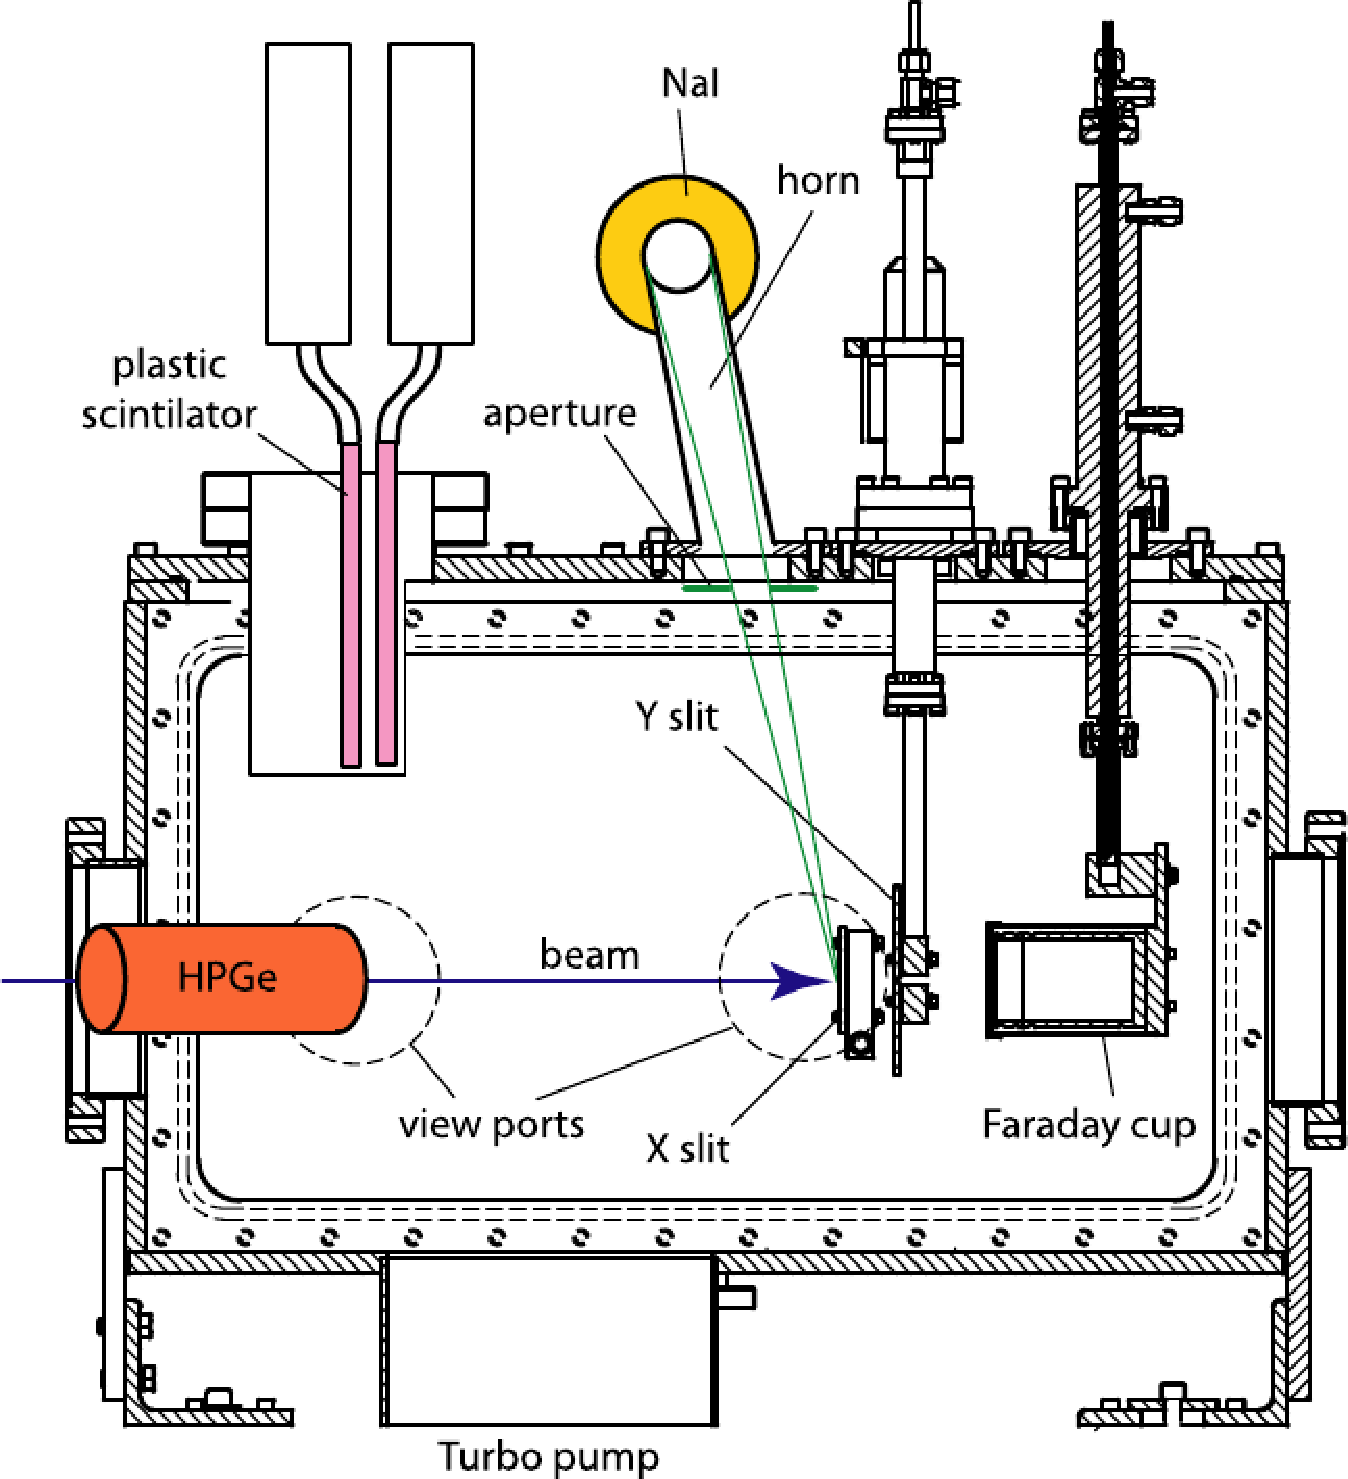
\includegraphics{Vockenhuber08_Fig3_XSLITM-chamber.pdf}
}
\caption{Radiation detectors at the DRAGON mass slits chamber. Two plastic scintillators are mounted inside a recess with a thin stainless steal wall on the side facing the mass slits. The HPGe detector (located external to the chamber) points at the mass slits through a view port, while the two NaI detectors are positioned about the `horn' and oriented at $180^\circ$ to each other. Taken from \cite{vock08}.}
\label{fig:xslitm}
\end{figure}
%
Care has to be taken, however, that different beam focussing does not affect detection efficiencies (through different deposit size or location). Additionally, the use of temporary beam intercepts is always possible, monitoring either charge or scattering in the moment of intercept, or radioactive decay of the material deposited in the non-intercept position. For example, regular Faraday cup measurements can be correlated to elastic scattering in the target, thus calibrating first the elastic scattering intensity to measured beam intensity, and subsequently normalizing the beam during the reaction measurement using the elastic scattering \cite{dau04}. 

\subsection{Prompt $\gamma$ ray detection}

Detection of prompt $\gamma$ rays by itself is a common method of determining reaction rates. $\gamma$-ray detectors are placed around a target to measure the decay lines from reaction products. This enables identification of $\gamma$ cascades and thus determination of branching ratios. This method has, however, the disadvantage of an often large background that has to be distinguished from the signal. It is thus often not possible to determine what fraction of the spectrum is due to the reaction under investigation. Combined with a recoils separator, however, prompt $\gamma$ detection at the target can be a valuable part of particle identification. $\gamma$ tagging can be used to improve the separator's background suppression by only including events with a valid $\gamma$ detection in the analysis. In conjunction with a focal plane detector, the time of flight (TOF) through the separator can be measured with the $\gamma$ event as the start signal and the focal plane detection as a stop signal (or vice versa using an appropriate delay). Using such TOF-based PID is especially advantageous when the background suppression of the separator decreases at lower energies \cite{hutc08}. 

Just as $\gamma$ tagging reduces the background in the focal plane detector, focal plane detection also reduces, and even eliminates, the background in the $\gamma$ spectrum. It is thus possible to determine the branching ratios using essentially background-free $\gamma$ spectra.\\
An additional benefit of placing $\gamma$ detectors around the target is their use in focussing the beam through the target. If the beam is poorly aligned, it can induce reactions or be deposited at the target entrance and exit aperture or on the target frame leading to increased $\gamma$ background. This background can be used as in indicator of the beam's misalignment.

Due to the typically low yields the main concern for $\gamma$ detectors in nuclear astrophysics is high efficiency. Specifically, the photo-peak efficiency needs to be high if the $\gamma$ detection is to be used to determine branching ratios. The cross section of the photo-effect varies with $\sigma_\mathrm{photo} \propto Z^{4\textrm{--}5}$, while Compton scattering goes with $\sigma_\mathrm{C} \propto Z$, and the probability for pair production as $\sigma_\mathrm{pair} \propto Z^2$. A high photo-peak efficiency therefore requires high-$Z$ materials. On the other hand, the ideal detector also has to cover a large range of energies. Reaction $Q$-values of several MeV mean that the recoil can be in states with several MeV excitation energy. Thus, a reasonable efficiency up to $\approx 10\unit{MeV}$ is required.

The fact that the $\gamma$ spectrum is essentially background free\footnote{With the exception of room background, which can be on the order of 0.1 kHz for an appropriately triggered array of BGO, for example. In addition, Coulomb-excitation of beam ions impinging on separator aperture can give rise to background $\gamma$ rays.} leads to somewhat less stringent requirements on the energy resolution. \\
The best energy resolution can be achieved using high-purity germanium (HPGe) detectors. They have, however several disadvantages. One is the relatively high cost of HPGe crystals compared to scintillator materials, another is the need for cooling, which leads to a less compact setup and additional maintenance costs. As an alternative to HPGe various scintillator materials are used for $\gamma$ detection. NaI(Tl) has a very high light output, and thus potentially good energy resolution. However, because of its low density of $3.67\unit{g/cm^3}$ it has a relatively low photopeak efficiency. In addition, it is hygroscopic, thus requiring the crystal to be sealed. Due to its high density of $7.13 \unit{g/cm^3}$, BGO (bismuth germanate) has a high photopeak efficiency. Thus, relatively small crystals can be used. Another commonly use scintillator material is BaF$_2$. Like BGO, BaF$_2$ is an intrinsic scintillator which does not require an activator. The still relatively high mass number of Ba ($Z = 56$) leads to a good photopeak efficiency. Wisshak et al. \cite{wiss84} compared the efficiencies of BGO and BaF$_2$ in an energy range from 0.5 to 10 MeV and concluded that an efficiency of 95\% would require either BGO with a thickness of 10 cm or BaF$_2$ with a thickness of 17.5 cm. Table \ref{tab:gamma_detectors} shows a comparison of some of the relevant properties of scintillation-based counters.



\begin{table*}
\label{tab:gamma_detectors}
\centering
\begin{tabular}{l|llll}
\hline
 & NaI(Tl) & BGO & BaF$_2$ & LaBr$_3$(Ce) \\
\hline
Density [$\mathrm{g/cm^3}$] & 3.67  & 7.13 & 4.88 & 5.1 \\
Hygroscopic & yes & no & slightly & yes\\
Light yield [photons/keV$\gamma$] & 38 & 8--10 & 10 (slow) & 63 \\
                                  &    &       & 1.8 (fast) &\\
Primary decay time [ns] & 250 & 300 & 630 (slow)  & 16\\
                        &     &     & 0.6 -- 0.8 (fast) &\\
\hline
\end{tabular}

\caption{Comparison of pertinent properties of various scintillation-based $\gamma$-ray detectors considered for use in recoil separators.}
\end{table*}


\subsection{Silicon strip detectors}
Silicon detectors are commonly employed as recoil detectors in the separator focal plane, their compact structure making them convenient to use. Due to the large number of charge carriers (the creation of one electron-hole pair requires 3.6 eV \cite{kemm88}) they provide good energy resolution in charged particle detection. With a pulse rise time of about 10 ns, good timing resolution is another advantage of silicon detectors, which, combined with a fast signal from {\it e.g.} a prompt $\gamma$ detector, enables precise time-of-flight measurements. \\
One disadvantage of silicon detectors is their sensitivity to radiation damage. Care must be taken not to expose them to high rates, especially of heavy particle radiation.\\
In addition to energy resolution, position resolution can be achieved by using microstrip detectors, (see Fig.\ \ref{fig:microstrip} \cite{rade84}).
%
\begin{figure}
\centering
\resizebox{0.95\columnwidth}{!}{
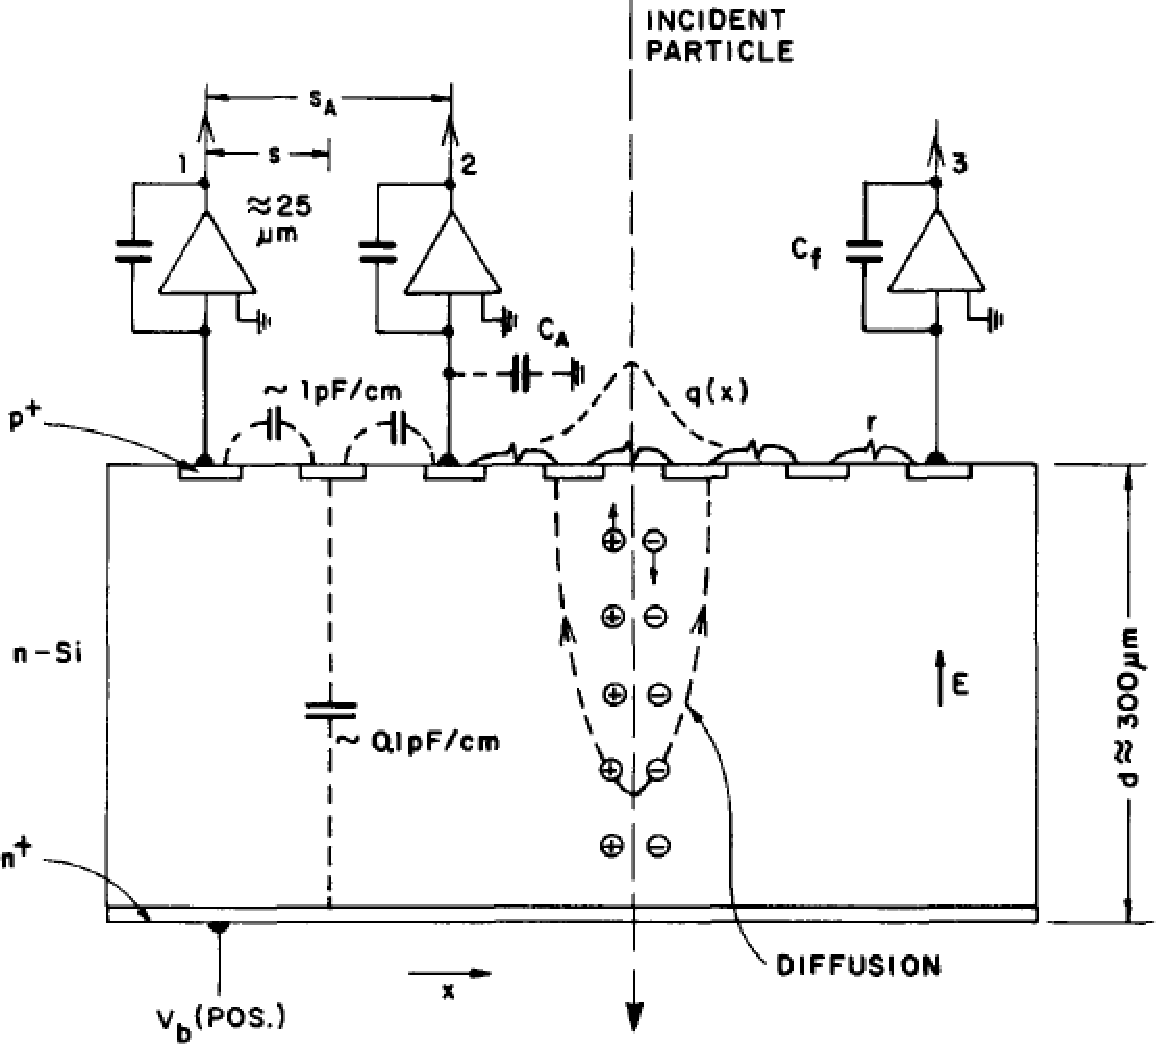
\includegraphics{Radeka84_Fig2_MicrostripDetector_PositionInterpolation.pdf}
}
\caption{Schematic representation of position interpolation in microstrip detectors. Diffusion spreads the charge [distribution $g(x)$] and determines maximum strip pitch $s$ for linear interpolation by centroid finding. Readout interpolation by capacitive charge division is illustrated between amplifiers 1 and 2. Resistive charge division is illustrated between amplifiers 2 and 3. Taken from \cite{rade84}.}
\label{fig:microstrip}
\end{figure}
%
Double-sided silicon strip detectors (DSSSDs) provide 2-dimensional position resolution by reading out perpendicular strips on the front and back of the detector. Position resolution can aid in particle identification if the recoil and the `leaky' beam follow different trajectories, but requires more electronics channels. Silicon detectors can also be stacked to form $\Delta{}E-E$ telescopes enabling particle identification by mass. However, the additional dead layers between the $\Delta{}E$ and $E$ detectors lead to a reduced energy resolution.\\  
Depending on the reaction kinematics, a $\Delta{}E-E$ telescope may require a very thin $\Delta{}E$ detector. This causes problems with mechanical stability and increases the production cost. Monolith silicon detectors avoid this problem by integrating both detectors into one unit \cite{card96}. A thin $\Delta{}E$ layer is implanted onto a thick silicon detector. An example of such a device is shown in Fig.\ \ref{fig:monolith}, taken from Ref.\ \cite{tudi99}. Position resolution is achieved by constructing the thin layer as separate pixels, each with separate readout electronics. Thus, the number of channels required for a monolith detector is larger than for a DSSSD. In addition, the large capacitance of the thin layer leads to a poor signal-to-noise ratio. Special preamplifiers are required to overcome this problem.%
%
\begin{figure}
\centering
\resizebox{0.95\columnwidth}{!}{
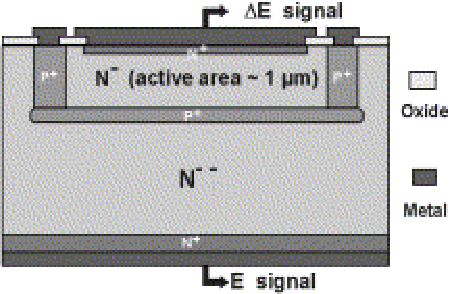
\includegraphics{Tudisco99_Fig1_monolith_sideview}
}
\caption{Side view of a monolithic silicon detector. Taken from \cite{tudi99}.}
\label{fig:monolith}
\end{figure}
%

\subsection{Ionization chambers}
At low energies ionization chambers (ICs) can be advantageous compared to silicon detectors, since a thin dead layer can be achieved by using an appropriately thin window. At such energies, the pressure inside the IC can be low while still stopping the particle in the active volume, allowing for the use of a thin window of sufficient size. Another advantage is that ICs are relatively low cost and, due to the lack of a solid structure, resistent to radiation damage.\\
The anode of an IC may be segmented, thus providing $\Delta{}E-E$ (often with several $\Delta{}E$ stages) particle identification. While the gas pressure can be adjusted to fit the beam and reaction product and their respective stopping powers, and thus optimise the resolution, the energy resolution is still inferior to that of a silicon detector. This is largely due to the lower number of charge carriers created by the incident particle; in most common gases, the energy required to create an electron-ion pair is about 25 -- 45 eV/pair (compare to 3.6 eV per electron-hole pair in silicon).\\
The timing resolution depends on the drift time of the electrons to the anode, which in turn depends on the geometry of the chamber, the drift gas, and the applied voltages. The drift time is usually of the order of $\unit{\mu{}s}$, leading to a timing resolution inferior to that of silicon detectors. 
ICs are in use at several recoil separator facilities. The DRAGON IC is shown in Fig.\ \ref{fig:ICs}. In this case, not only can the gas pressure be adjusted, but the widths of the anodes can be changes in steps of 1 cm, using up to 5 anodes total.
Alternatively, with an unsegmented anode, the IC can function as a $\Delta{}E$ stage with a silicon detector mounted at the back as the $E$ detector. Such a setup was used, {\it e.g.} at ARES \cite{coud03}, and is shown in the top panel of Fig.\ \ref{fig:ICs}.
\begin{figure}
\centering
\resizebox{0.8\columnwidth}{!}{%
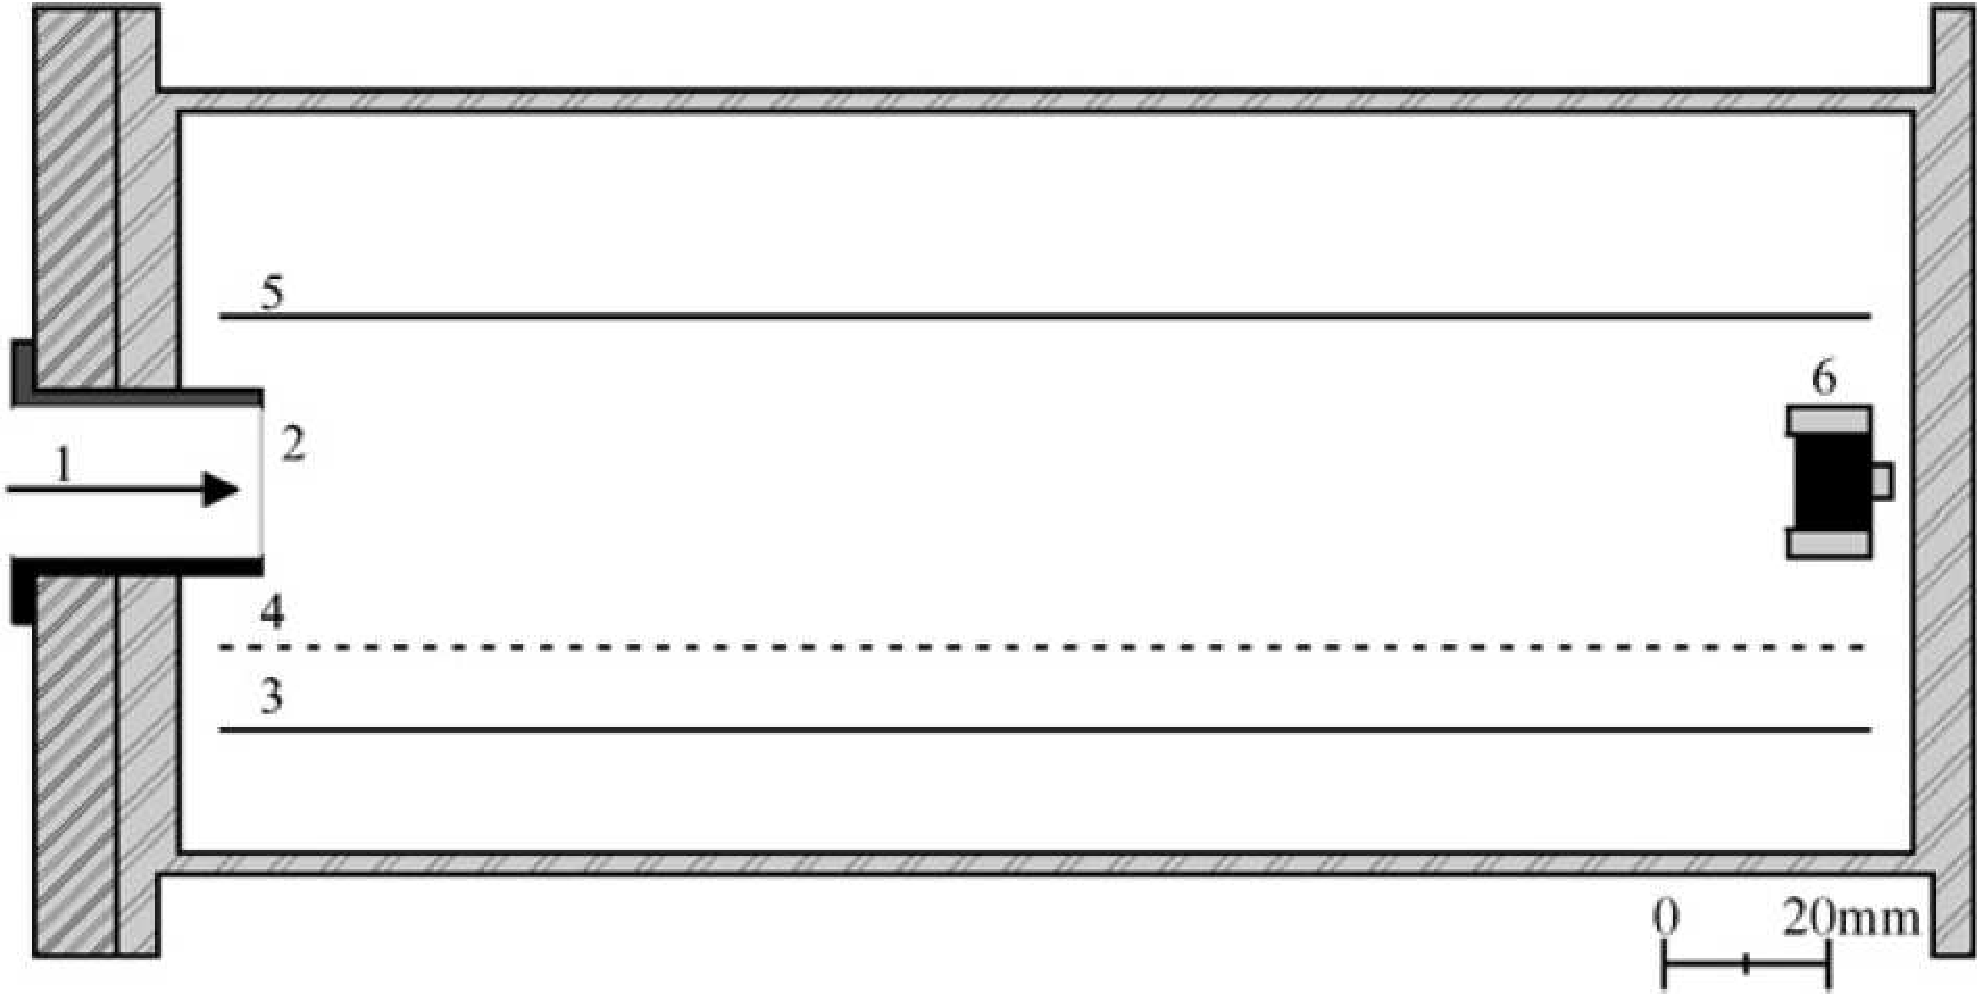
\includegraphics{Couder03_Fig5_ARES-IC}
}
\resizebox{0.98\columnwidth}{!}{%
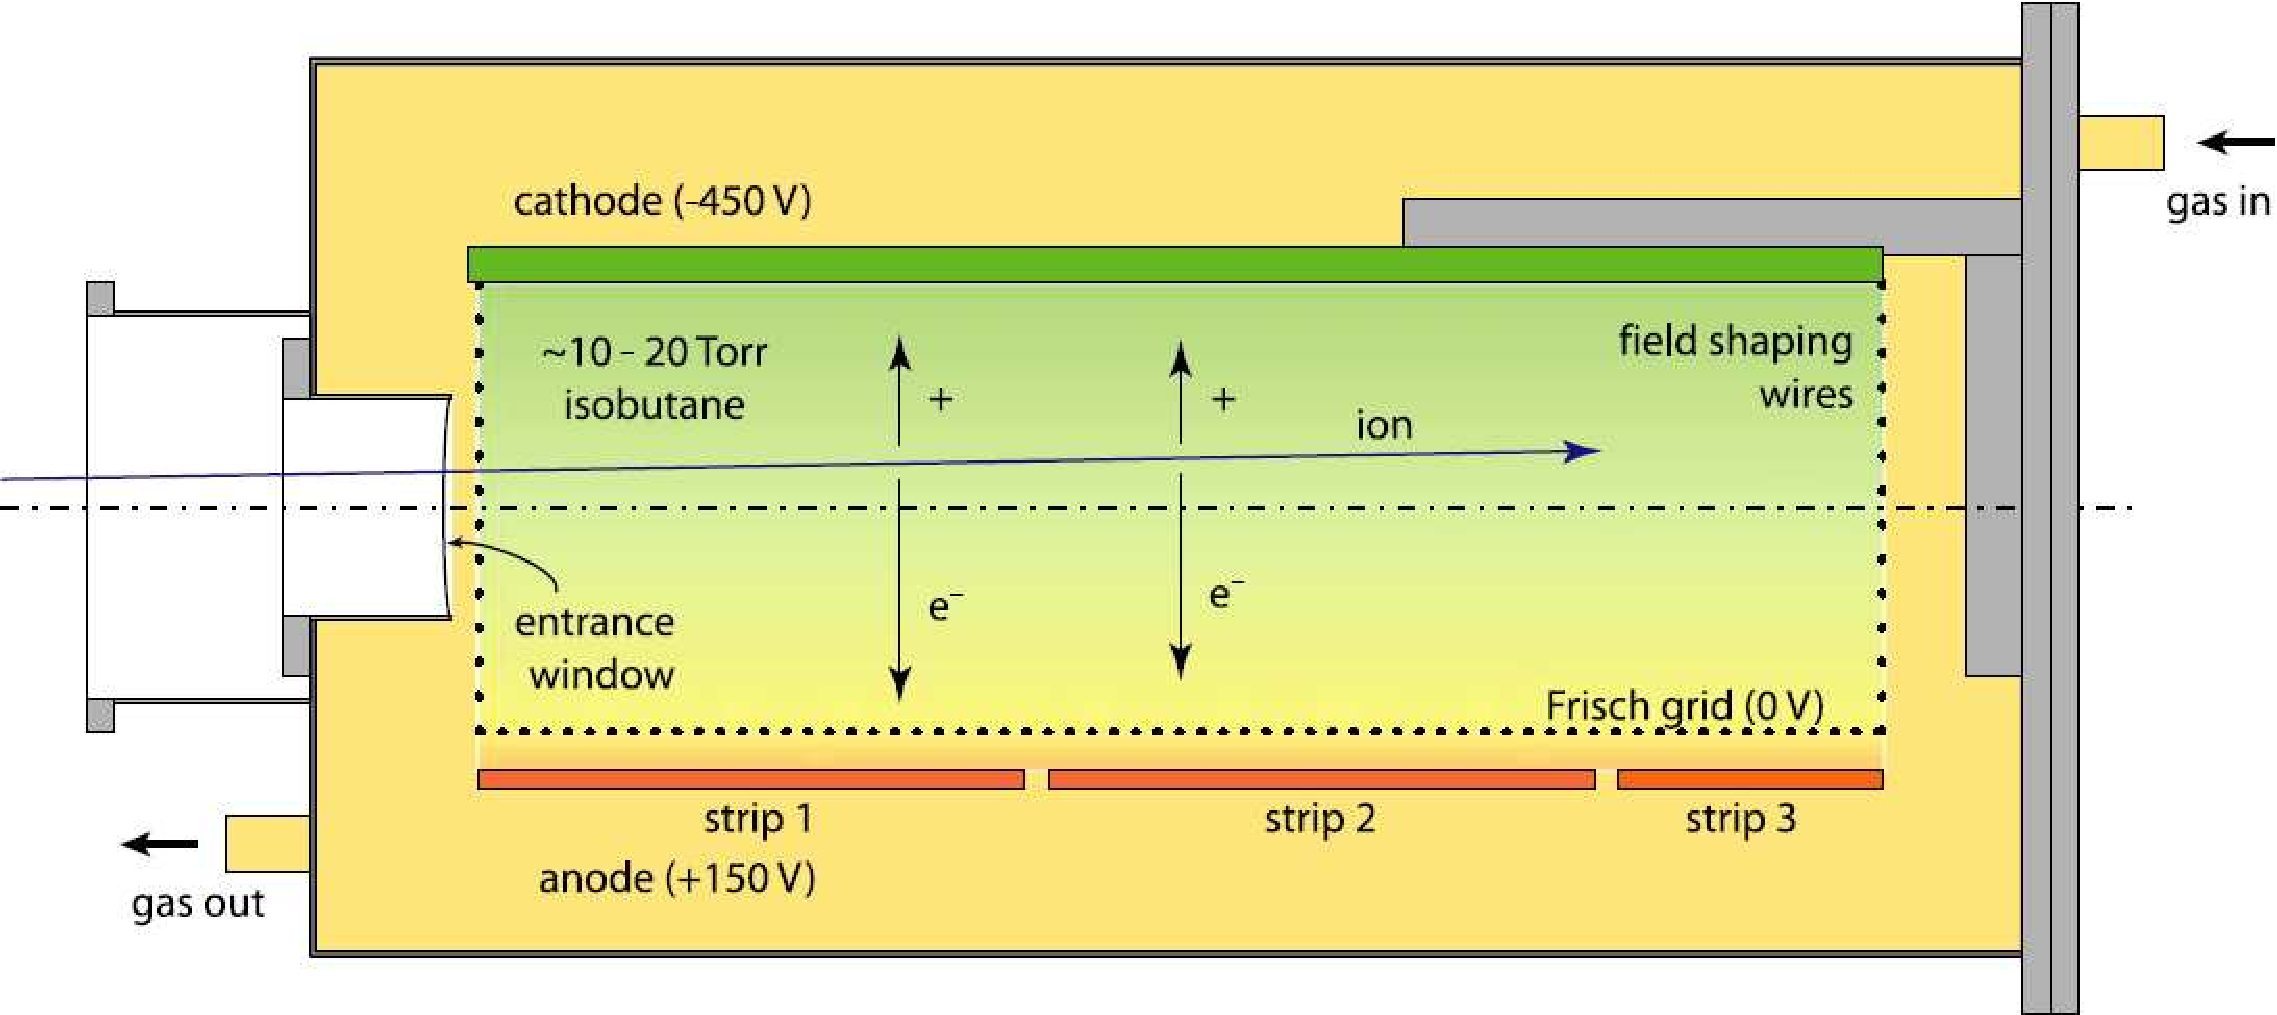
\includegraphics{Vockenhuber08_Fig4_DRAGON-IC}
}
\caption{Drawings of the ARES (upper) and DRAGON (lower) ICs. Taken from \cite{coud03,vock08}.}
\label{fig:ICs}
\end{figure}


\subsection{Local time-of-flight}

Non-destructive time-of-flight measurement provides good resolution at lower energies, where the IC and DSSSD resolutions decrease. This is especially important as the beam suppression of the separator generally decreases with decreasing energy \cite{hutc08}. The advantage of a non-destructive measurement is that it can be combined with PID in a focal plane detector. The measurement should thus interfere as little as possible with the particles' energy and trajectory. In addition, the resolution must be sufficient to distinguish reaction recoils from beam particles. From this follow requirements for the detectors' timing resolution and hence the minimum distance between them. In typical \reac{p}{\gamma} and \reac{\alpha}{\gamma} reactions in nuclear astrophysics, the recoil velocity is usually between 75 and 95\% of the beam velocities, with beam velocities of around $10^7 \unit{m/s}$.   \\
One way to meet the requirements is to use microchannel plate (MCP) detectors to detect secondary electrons emitted when the beam passes through a thin foil \cite{star82}. The secondary electrons can be deflected into the MCP using wire planes at appropriate potentials, as shown in Fig. \ref{fig:Starzecki82_Fig1}.
%
\begin{figure}
\centering
\resizebox{0.98\columnwidth}{!}{
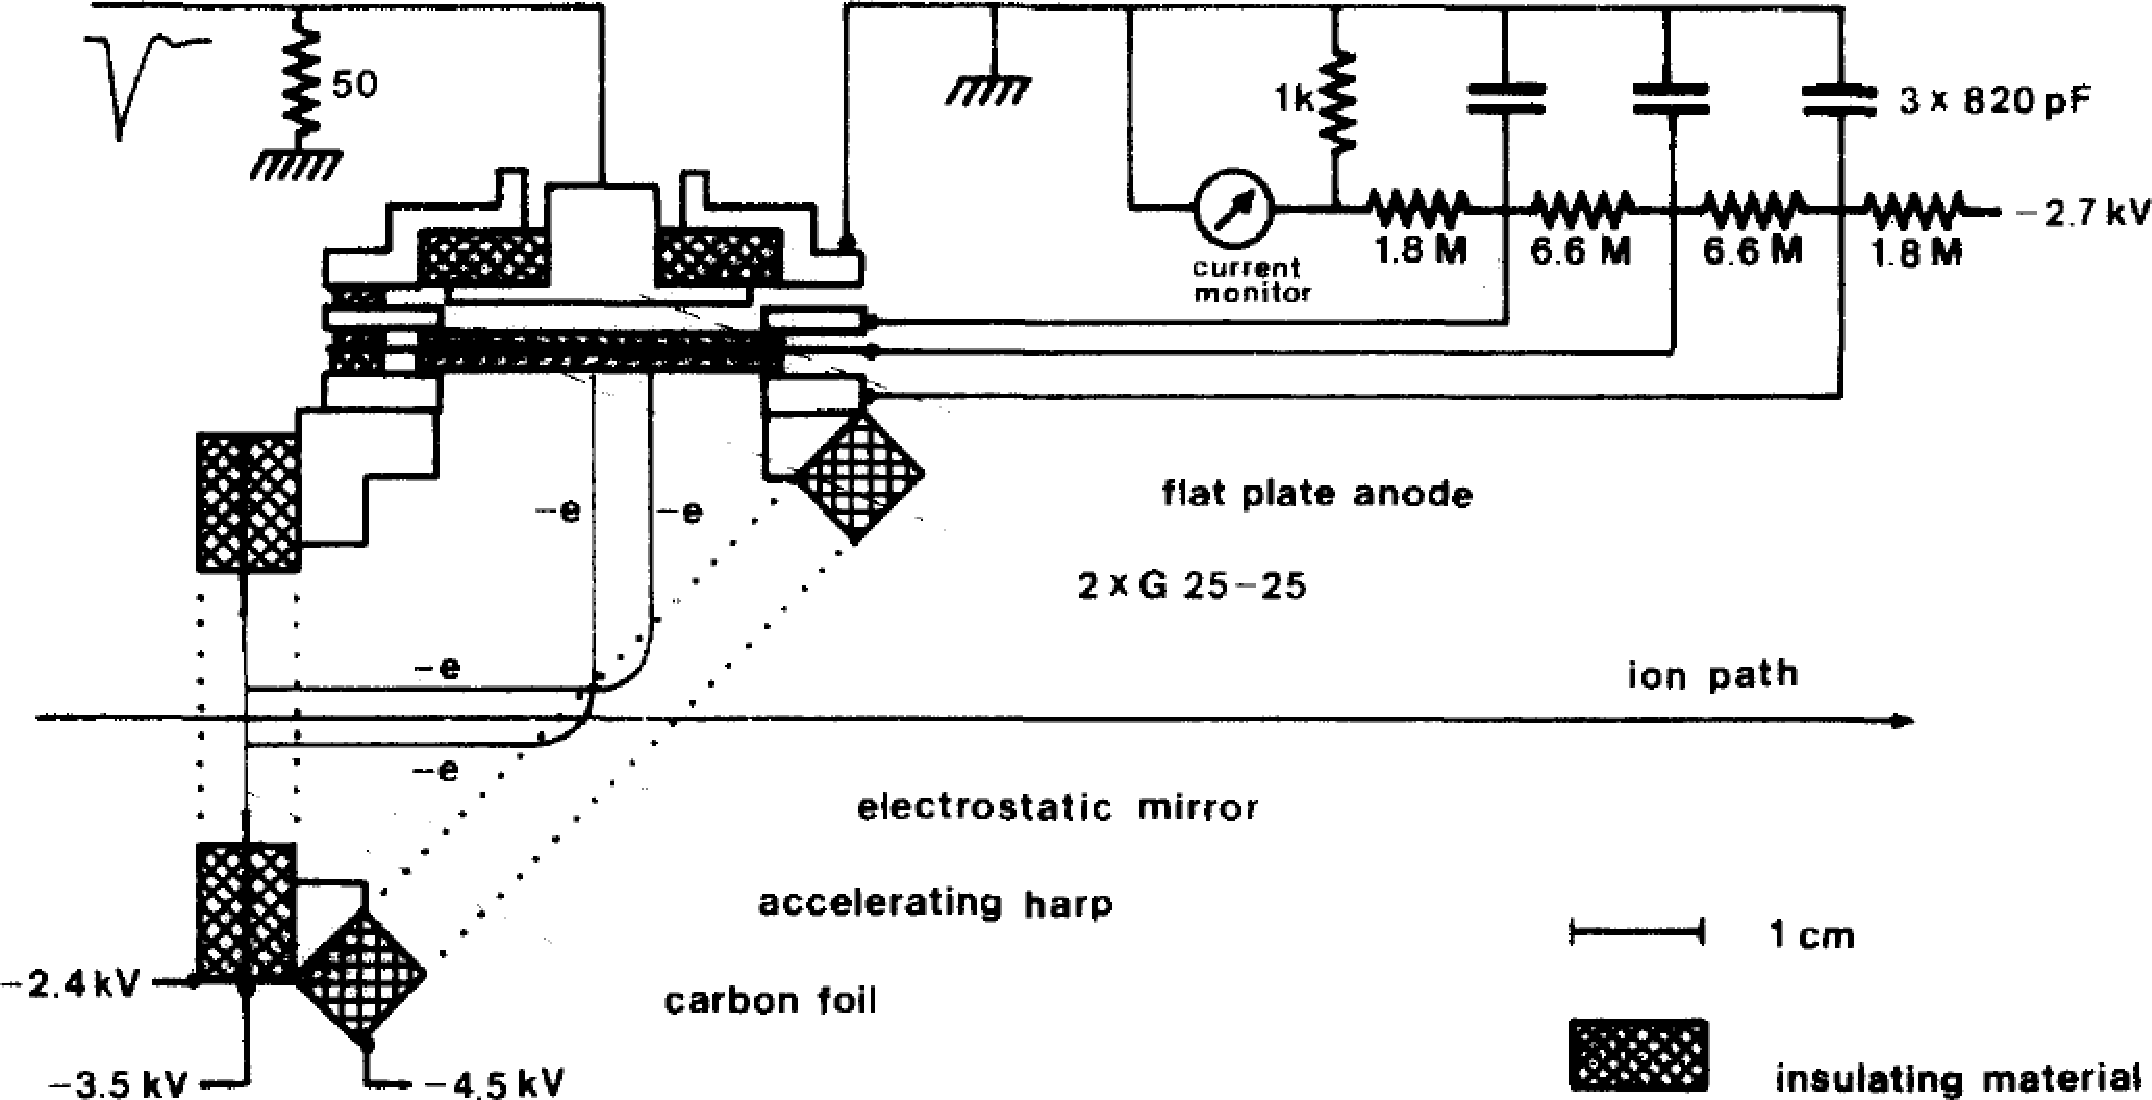
\includegraphics{Starzecki82_Fig1_TimeZeroDetector.pdf}
}
\caption{Schematic view of the time-zero detector. With the potentials indicated here the reflection of the electrons occurs 1.5 mm inside the mirror. Taken from \cite{star82}.}
\label{fig:Starzecki82_Fig1}
\end{figure}%
%
The MCP itself can thus be mounted outside the beam path. MCP detectors have a very good timing resolution of around 100 ps. They can also be build using resistive anodes and thus enabling position measurement. If the trajectories of the reaction products and the beam particles differ, this position can be used as an additional PID parameter. Using two such setups separated by 59 cm, timing resolutions of better than 400 ps have been demonstrated \cite{vock09}. \\
The efficiency of the foil-MCP system depends on how many secondary electrons are emitted from the foil when the charged particle passes through. This number depends on the stopping power $dE/dx$ and is thus larger for heavier ions. In addition, the electron multiplication in the MCP and the electronic threshold influence the detection efficiency.\\
The thickness of the foils is limited by the required energy resolution in the focal plane detector. Thinner foils are desirable, but difficult to float on frames with large apertures, which are required to cover the different trajectories of recoil ions and scattered beam. Thus, the foils are often mounted on meshes \cite{vock09}. Still, pin-holes can cause reduction in the detection efficiency. The meshes also reduce the transmission of the TOF system, as do the electrostatic mirror wire planes. 


